%Capitulo V Conclusión/Valoración de objetivos


%Para terminar es necesario revisar los objetivos planteados, verificar su cumplimiento y en caso de no haberse cumplido justificar el por que no se pudo cumplir el objetivo.


\chapter{ CONCLUSIÓNES }

\section{Características finales de la tarjeta}

\begin{figure}[H]
	\begin{center}
 		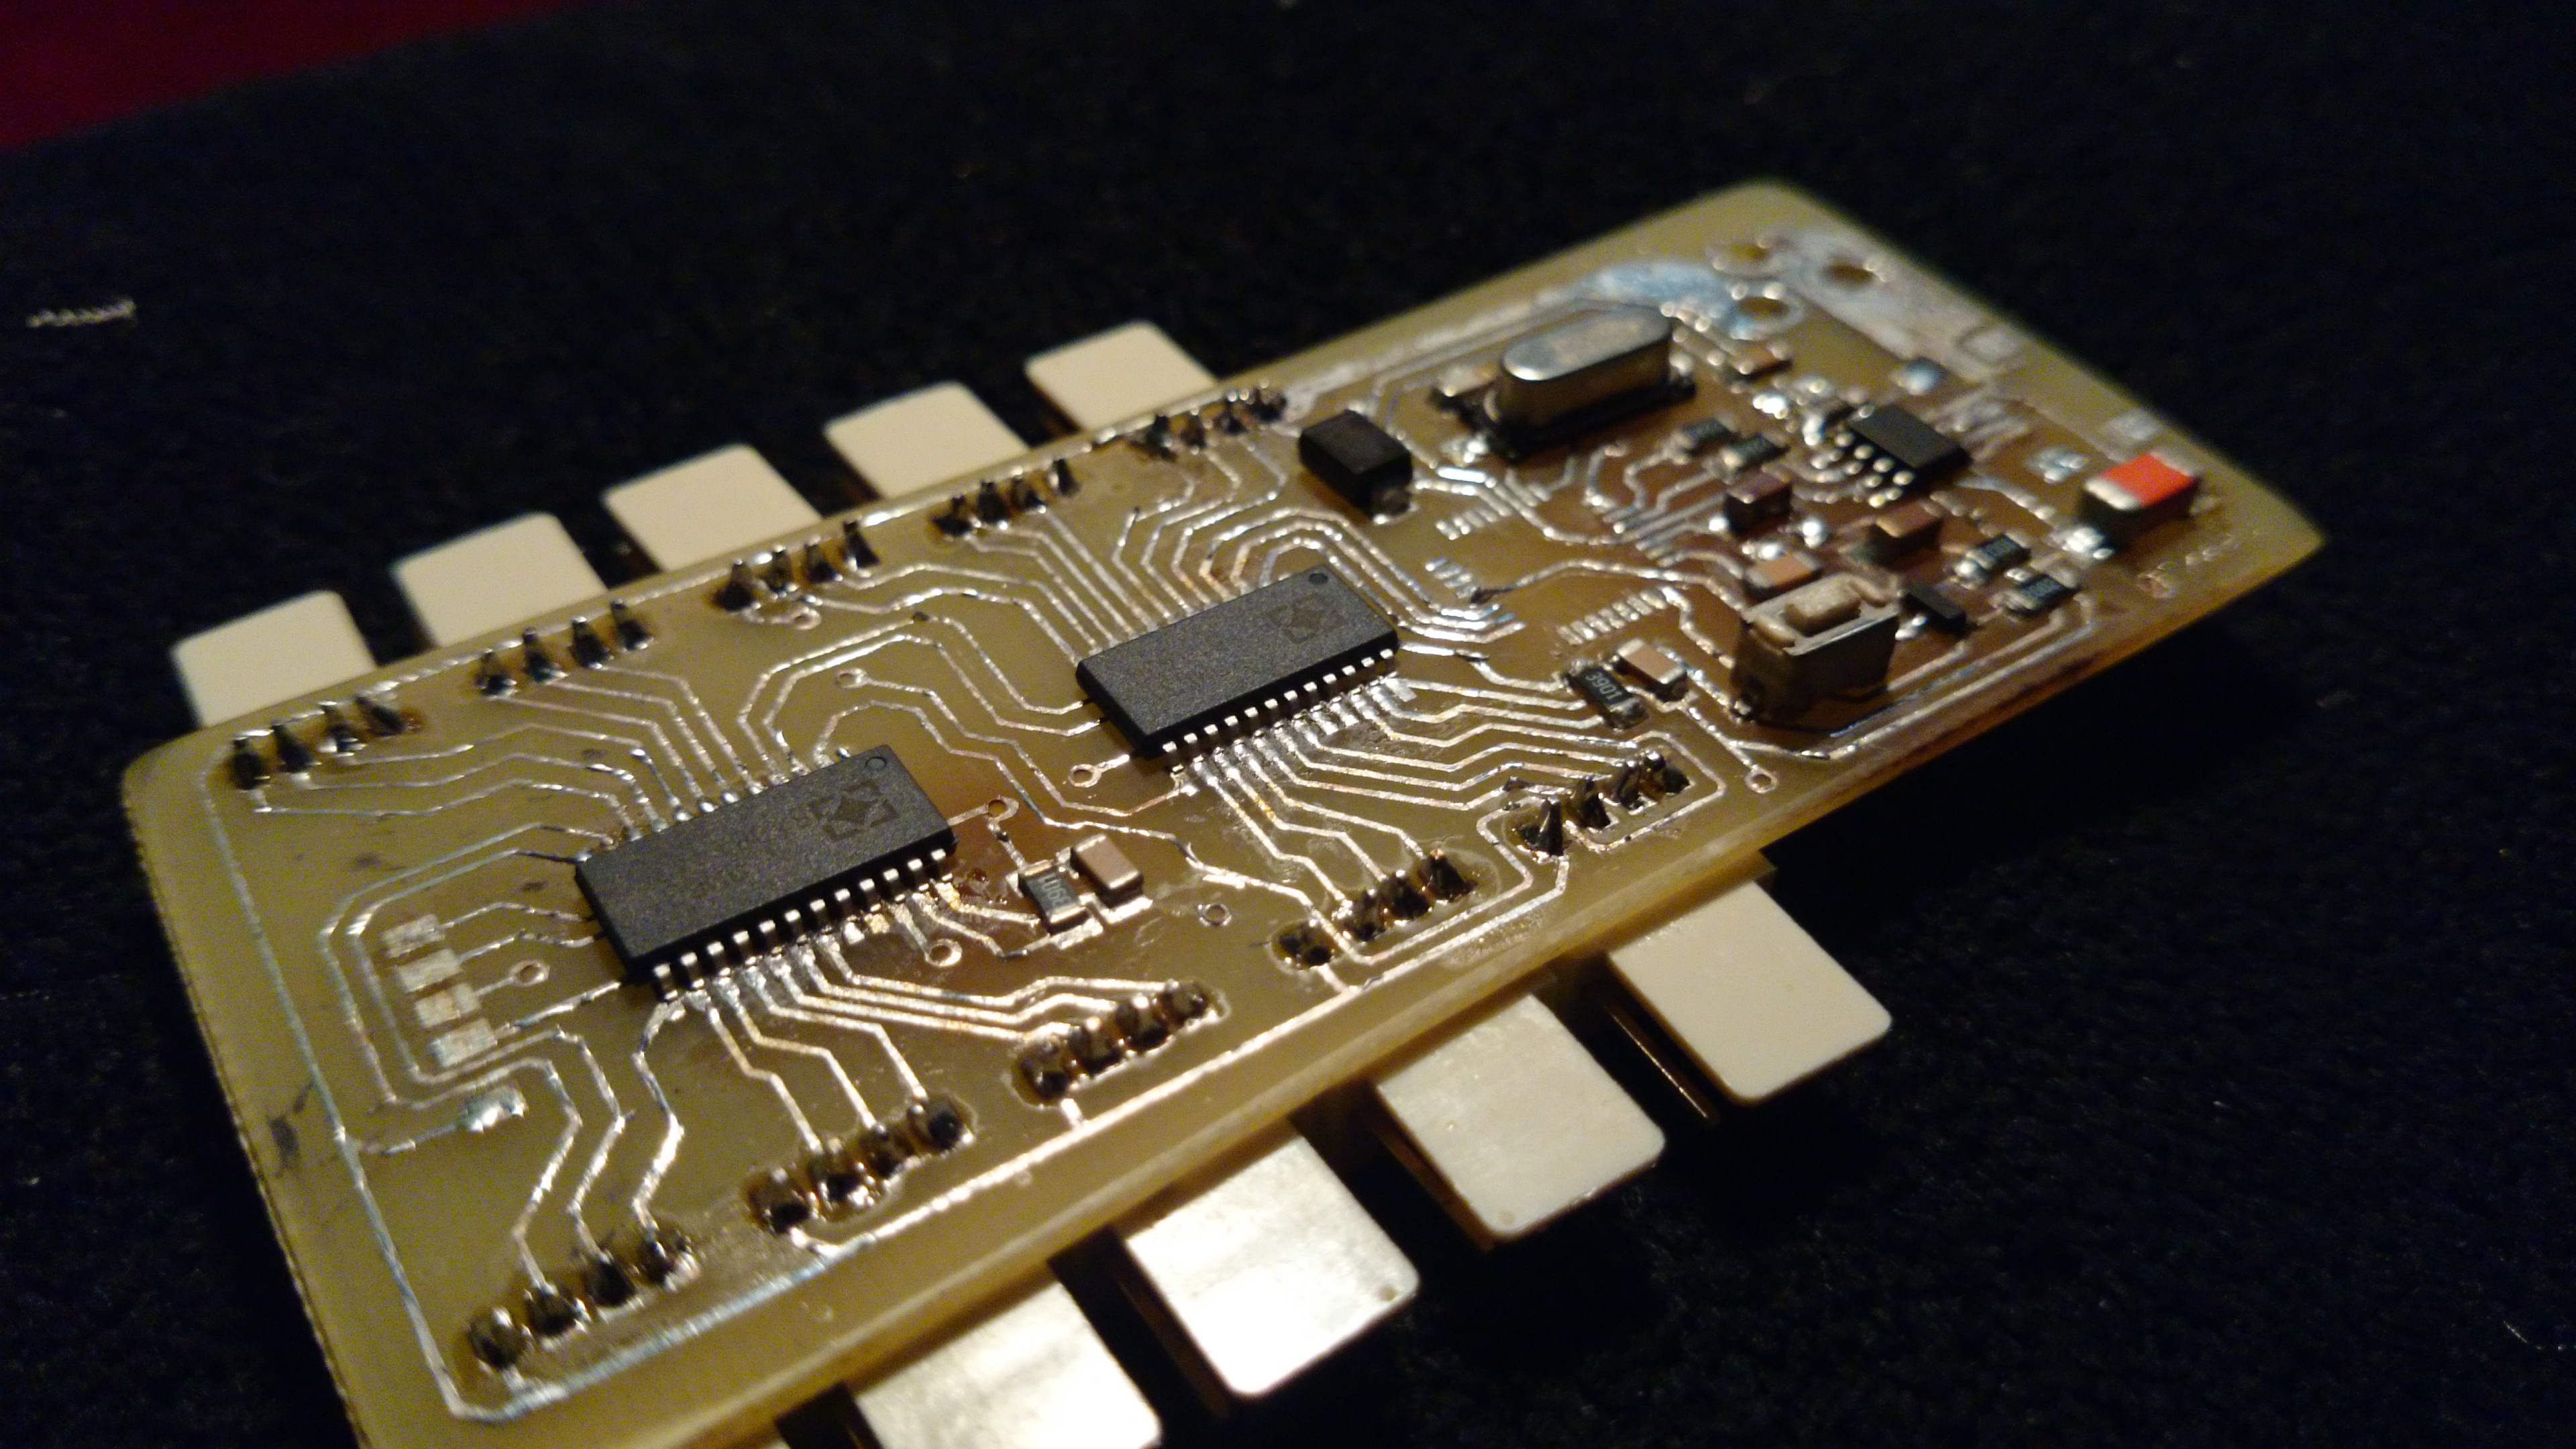
\includegraphics[width = .65\textwidth]{Tesis/Imagenes/prototipo.jpg}
 		\captionof{figure}{Tarjeta de Circuito Impreso finalizada}
	\label{prototipo}
    \end{center} 
\end{figure}


\section{ Comparación con sistemas existentes }

\textit{Utilizando los resultados obtenidos en el capitulo VI (Análisis) es ahora posible cotejar la información y ponerlos uno contra otro para hacer una comparación de los sistemas existentes contra el sistema generado.}


\section{ Análisis costo-beneficio }

\textit{Es necesario justificar la relación costo beneficio del proyecto}

\section{ Trabajo futuro }

\textit{En esta sección caben todas aquellas ideas o mejoras que en algún momento a lo largo del proyecto se pensaron implementar pero no se contemplaron en los objetivos principales o que no tuvieron cabida dentro del lapso de tiempo en el que se desarrolla el proyecto.} 


\section{ Conclusiones }

\textit{Como se observa, desarrollar y redactar un Proyecto y un documento de Tesis, no es una actividad fácil.}

\textit{Conlleva una voluntad férrea, así cómo: una filosofía, mentalidad y aplicación sistémica y sistemática de los conocimientos adquiridos a lo largo de los cursos y del mismo desarrollo del proyecto que, en ocasiones, no sólo es la cúspide de los estudios, sino su reafirmación y mayor integración} \cite{Leopoldo}.




%Capitulo V Conclusión/Valoración de objetivos